\documentclass[12pt,letterpaper]{article}
\usepackage[utf8]{inputenc}
\usepackage{float, xcolor}

%----- Configuración del estilo del documento------%
\usepackage{graphicx, fancyhdr, lastpage}
\usepackage[left=2cm,right=2cm,top=1.8cm,bottom=2.3cm]{geometry}

\pagestyle{fancy}
\fancyhf{}
\rfoot{\textit{Página \thepage \hspace{1pt} de \pageref{LastPage}}}

%------ Paquetes matemáticos básicos --------%
\usepackage{amsmath, amssymb, amsthm}

\newcommand{\imp}{\rightarrow}

\begin{document}

%------ Encabezado -------- %
\begin{center}
  \begin{minipage}{3cm}
    \begin{center}
      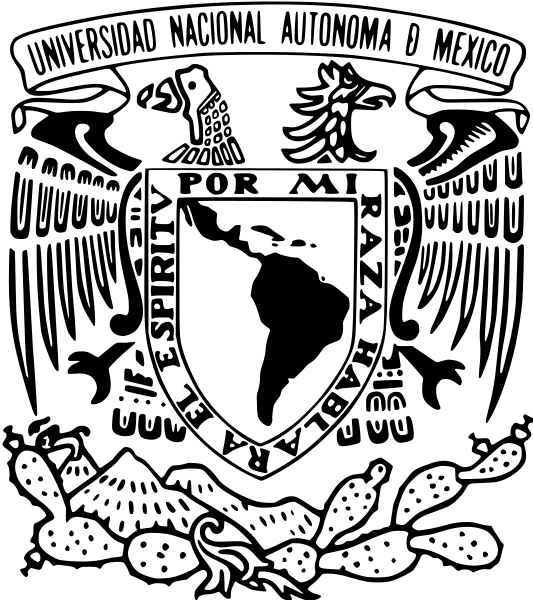
\includegraphics[height=3.4cm]{unam_logo.png}
    \end{center}
  \end{minipage}\hfill
  \begin{minipage}{10cm}
    \begin{center}
      \textbf{\Large Universidad Nacional Autónoma de México}\\[0.2cm]
      \textbf{\large Facultad de Ciencias}\\[0.2cm]
      \textbf{Lógica Computacional | 2025-2}\\[0.4cm]
      \textbf{\Large Tarea 01}\\[0.1cm]
      \textbf{Docentes:}\\
      Noé Hernández \hspace{1em} Santiago Escamilla \hspace{1em} Ricardo López\\[0.3cm]
      \textbf{Autores:}\\
      Fernanda Ramírez Juárez \quad Ianluck Rojo Peña\\[0.3cm]
      \textbf{Fecha de entrega:} Miércoles 12 de febrero de 2025
    \end{center}
  \end{minipage}\hfill
  \begin{minipage}{3cm}
    \begin{center}
      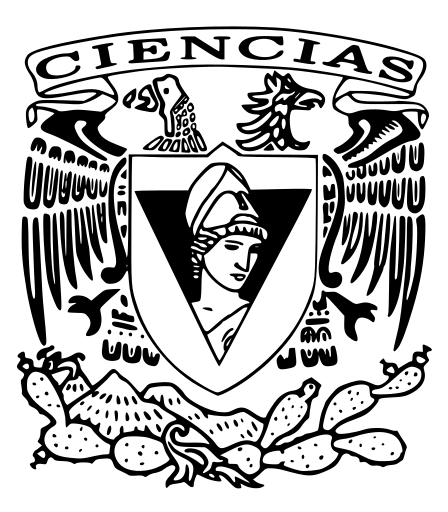
\includegraphics[height=3.4cm]{fc_logo.png}
    \end{center}
  \end{minipage}
\end{center}

\bigskip
\hrule height 0.1pt
\bigskip

%------ Notas sobre la resolución --------%
\section*{Notas sobre la resolución}

\begin{quote}
  \textbf{Nota general:}  
  Los ejercicios fueron resueltos en base a las notas de clase (IcNota2.pdf) y a los comentarios dados en las sesiones del curso. Se tomaron en cuenta los siguientes puntos específicos:  
\end{quote}

\begin{itemize}
   \item \textbf{Ejercicios :}
\end{itemize}

\bigskip
\hrule height 0.1pt
\bigskip

%------ Contenido -------- %
\section*{Resolución de Ejercicios}

\begin{enumerate}
  
  % ---- Ejercicio 1 ----
  \item (1.5 pts.) El sumador que aparece abajo implementa el par de fórmulas:
    \begin{multicols}{2}
      \begin{center}
	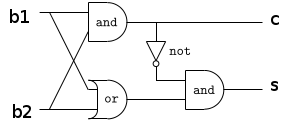
\includegraphics[scale=0.9]{circuit}
      \end{center}

      \[
      s \leftrightarrow \neg(b_1\wedge b_2)\wedge (b_1\vee b_2), \qquad c\leftrightarrow b_1\wedge b_2.
      \]
    \end{multicols}
Sea $C$ el conjunto que contiene al par de fórmulas anteriores. Usando resolución binaria, muestre que $C\cup\{b_1 \wedge\, b_2 \wedge\, \neg s \wedge\, \neg c\}$ genera un conjunto insatisfacible, mientras que $C\cup\{b_1 \wedge\, b_2 \wedge\, \neg s \wedge\, c\}$ genera un conjunto satisfacible. Explique lo que esto significa en términos del comportamiento del circuito.

  % ---- Ejercicio 2 ----
\item (1.5 pts.) ¿Es el siguiente conjunto de fórmulas satisfacible? Utilice resolución binaria para contestar esta pregunta.
\[
\{
(p\imp r)\vee (\neg s\wedge p), s\imp\neg(p\wedge r), r\vee s
\}\]


  % ---- Ejercicio 3 ----
\item (2 pts.) Compruebe la validez del siguiente argumento lógico usando resolución binaria.

{\it Si Batman es el más popular de los superhéroes, entonces Superman ha muerto. Si Superman ha muerto, la Mujer Maravilla preside la Liga de la Justicia. Si la Mujer Maravilla preside la Liga de la Justicia, Batman es el más popular de los superhéroes. Por lo tanto, Superman no ha muerto si y sólo si Batman no es el más popular de los superhéroes.}

Use las siguientes claves:
\begin{itemize}[label={--}]
    \item $b$: Batman es el más popular de los superhéroes
    \item $s$: Superman ha muerto
    \item $m$: La Mujer Maravilla preside la Liga de la Justicia
\end{itemize}

  % ---- Ejercicio 4 ----
\item (1.5 pts.) Demuestre el Lema 1.4 en la \href{https://drive.google.com/file/d/1neZfLRMBIsvz2ZycHT0h7z0lKTuAe6pv/view}{Nota 05}. \emph{Sea $S$ un conjunto de cláusulas y sea $C\in S$ una cláusula trivial. $S-\{C\}$ es lógicamente equivalente a $S$.}


  % ---- Ejercicio 5 ----
\item (1.5 pts.) Demuestre que una disyunción de literales $\ell_1 \vee \ldots \vee \ell_m$ es válida syss existen $1\leq i, j \leq m$ tal que $\ell_i$ es $\neg\ell_j$.


  % ---- Ejercicio 6 ----
\item (1 pts.) Realice las siguientes sustituciones:
\begin{enumerate}
\item $\Big(\forall x .\big( Q(w,y,x) \wedge P(f(x),w,b) \big) \Big)[y,w:=f(w),g(x)]$
\item $\Big(\begingroup\colorlet{savedleftcolor}{.}\color{red}\big(\color{savedleftcolor}\forall v .\forall w . \big( P (u, v, x) \wedge R(a, x) \wedge Q(u, w) \big)\color{red}\big)\endgroup [x, u := v, g(a, w)]\Big)[v:=f(y)]$
\end{enumerate}


  % ---- Ejercicio 7 ----
\item (1 pts.) ¿Cuál es la mejor traducción para: {\em Se siente bien feo cuando se muere algo adorable que querías mucho}? Donde: $S(x)$: $x$ se siente bien feo;  $M(x)$: $x$ se muere; $A(x)$: $x$ es adorable y $Q(x,y)$: $x$ quiere mucho a $y$.
	\begin{enumerate}
	\item $\forall x\Big(S(x)\vee \forall y\ \neg\big(M(y)\wedge Q(y,x)\wedge A(y)\big)\Big)$
	\item $\forall x\Big(\forall y \big(\neg M(y)\imp (Q(y,x)\imp \neg A(y))\big)\vee S(x)\Big)$
	\item $\forall x\Big(\neg S(x) \imp \forall y \big(M(y)\wedge Q(x,y)\imp\neg A(y)\big)\Big)$
	\item $\forall x\Big(\forall y\big(A(y)\wedge( Q(x,y) \wedge M(x)\big)\imp S(x)\Big)$
	\end{enumerate}

  % ---- Ejercicio 8 ----
\item (1 pt.) En una isla habitada por ingleses, funcionan tres clubes. ¿Cuál simbolización expresa mejor la siguiente afirmación? {\it Cualesquiera dos clubes tienen un socio en común.} Donde: $C(x)$: $x$ es un club; $S(x,y)$: $x$ es socio de $y$.
	\begin{enumerate}
	\item $\exists x\  \exists y\ \exists z\ \big(x\neq y \wedge C(x) \wedge C(y) \wedge S(z,x) \wedge S(z,y)\big)$
	\item $\exists z\ \forall x\  \forall y\ \big((x\neq y \wedge C(x) \wedge C(y)) \imp (S(z,x) \wedge S(z,y))\big)$
	\item $\forall x\  \forall y\ \big((x\neq y \wedge C(x) \wedge C(y)) \imp \exists z\ (S(z,x) \vee S(z,y))\big)$
	\item $\forall x\  \forall y\ \exists z\ \big((x\neq y \wedge C(x) \wedge C(y)) \imp (S(z,x) \wedge S(z,y))\big)$
	\end{enumerate}

\end{enumerate}

Para los dos últimos incisos tome en cuenta estas equivalencias:
\[\arraycolsep=1.4pt\def\arraystretch{1.5}
\begin{array}{lcl}
\vp \imp \psi &\equiv& \neg\vp \vee\psi\\
\vp \imp \psi &\equiv& \neg\psi \imp \neg\vp\\
\neg(\vp\wedge\psi) &\equiv& \neg\vp\vee\neg\psi\\
\neg(\vp\vee\psi) &\equiv& \neg\vp\wedge\neg\psi\\
\neg\forall x\;\vp &\equiv& \exists x\;\neg\vp\\
\neg\exists x\;\vp &\equiv& \forall x\;\neg\vp
\end{array}
\]

\end{document}
